\chapter{Разработка адаптивного к скорости движения ПА метода управления ДРК}\label{ch:Allocation}

% \section{Формальное описание структуры ДРК}\label{sec:Allocation/System}
% \begin{noteplan}
% 	Думаю эту секцию перенесу во вторую главу. А здесь оставлю только анализ матрицы геометрии ДРК.
% \end{noteplan}

% Движители в системе можно разделить на три больших класса \cite{армишев86}:
% \begin{itemize}
%     \item \textbf{фиксированные}, когда вектор упора может изменяться только вдоль фиксированной относительно ПА прямой.
%     \item \textbf{поворотные} (азимутальные, azimuth), когда вектор упора может изменяться в фиксированной относительно ПА плоскости.
%     Сюда относятся гребные винты на поворотных колонках, гребные винты с поворотными насадками, крыльчатые движители и т.д.
%     \item \textbf{пространственные}, когда вектор упора может изменяться в пространстве.
% \end{itemize}
% Следует отметить, что если первые два класса движителей были заимствованы для ПА с надводных судов, то пространственные движители были разрабтаны для решения специфических задач подводных аппаратов.

% Определим формально, как по структуре ДРК находится число степеней свободы $m$, которые можно контролировать движение данного ПА, и наоборот, какова должна быть структура ДРК, что бы можно было управлять по заданным степеням свободы.

% Пусть $Oxyz$ -- правая ортогональная система координат жестко связанная с ПА. Ось $Ox$ направлена из кормы в нос, ось $Oy$ с левого борта на правый, а ось $Oz$ дополняет систему до правой ортогональной (SNAME нотация системы координат).

% Введём следующие обозначения:
% \begin{itemize}
%     \item $n_f \geq 0, n_a \geq 0, n_r \geq 0$ -- число, соответственно, фиксированных, поворотных и пространственных движителей входящих в состав ДРК;
%     % \item $i$ -- номер по порядку каждого движителя, где $i$ меняется в диапазоне $1,2, \ldots, n_f+n_a+n_r$;
%     \item $u^{i}, i < n_f$ - величина упора фиксированного движителя;
%     \item $(u^{i}_x, u^{i}_y, u^{i}_z)$, где $i$ меняется в диапазоне $n_f+1, n_f+2, \ldots, n_f+n_a+n_r$ -- проекции векторов упоров поворотных и пространственных движителей, соответственно на оси $Ox, Oy, Oz$;
%     \item $(P^i_x, P^i_y,P^i_z)$ -- координаты точки крепления движителя с номером $i$ относительно $Oxyz$;
%     \item $(C^i_x, C^i_y, C^i_z)$ -- направляющие косинусы единичного вектора, направленного вдоль линии действия фиксированного движителя с номером $i$;
%     \item $(R^i_x, R^i_y, R^i_z)$, где $i$ меняется в диапазоне $n_f+1, n_f+2, \ldots, n_f+n_a$ -- направляющие косинусы вектора единичной нормали к плоскости вращения поворотного движителя с номером $i$;
%     \item $(\nu_x, \nu_y, \nu_z)$ -- проекции главного вектора управляющих сил на оси $Ox, Oy, Oz$;
%     \item $(\nu_{mx},\nu_{my},\nu_{mz})$ -- проекции главного вектора момента управляющих сил на оси $Ox, Oy, Oz$.
%     \item $\vect{u}=[u^{1}, u^{2}, \ldots, u^{n_f+n_a+n_r}_x, u^{n_f+n_a+n_r}_y, u^{n_f+n_a+n_r}_z]^T$ -- обобщенный вектор упоров создаваемый ДРК;
%     \item $\vect{\nu} = [\nu_x, \nu_y, \nu_z, \nu_{mx},\nu_{my},\nu_{mz}]^T$ -- обобщенный вектор сил и моментов действующий на аппарат в системе координат $Oxyz$.
% \end{itemize}

% Можно показать что между векторами $\vect{u}$  и $\vect{\nu}$ есть линейная зависимость, которая выражается через матрицу $B$:
% \begin{equation}
%     \label{eq:propulsion_connection}
%     B\vect{u} = \vect{\nu}
% \end{equation}

% В \ref{eq:propulsion_connection} шесть уравнений определяют связь между проекциями сил и моментов в связанной с аппаратом системе координат $Oxyz$ с одной стороны и $n_f$ упоров фиксированных и $3(n_r+n_r)$ проекций упоров поворотных и пространственных движителей с другой стороны.

% Однако не все создаваемые движителями упоры являются независимыми.
% Вектор тяги поворотного движителя должен всегда лежать в плоскости вращения. 
% Для этого вводят расширенный вектор сил и моментов $\vect{\nu^e} = [\vect{\nu}, 0, \ldots, 0]$, где $\vect{\nu^e} \in \mathspace{R}^{6+n_a}$ и соответствующую матрицу $B^e$:
% \begin{equation}
%     \label{eq:propulsion_connection_enchanced}
%     B^e\vect{u} = \vect{\nu^e}
% \end{equation}
% где последние $n_a$ уравнений отражают это ограничение накладываемое на вращательные движители.

% Общие вид матрицы $B^e=(B^e_f, B^e_a, B^e_r)$, где $B^e_f \in \mathspace{R}^{(6 + n_f) \times n_f}$ (\ref{eq:propulsion_matrix_fix}), $B^e_a \in \mathspace{R}^{(6 + n_f) \times 3n_a}$ (\ref{eq:propulsion_matrix_azimuth}), $B^e_r \in \mathspace{R}^{(6 + n_f) \times 3n_r}$ (\ref{eq:propulsion_matrix_rotation}) -- матрицы отражающая влияние фиксированных движителей, поворотных и пространственных движителей соответственно.

% \begin{equation}
%     \label{eq:propulsion_matrix_fix}
%     B^e_f = 
%     \begin{pmatrix}
%         C^1_x & \ldots & C^{n_f}_x \\
%         C^1_y & \ldots & C^{n_f}_y \\
%         C^1_z & \ldots & C^{n_f}_z \\
%         [C^1 \times P^1]_x & \ldots & [C^{n_f} \times P^{n_f}]_x \\
%         [C^1 \times P^1]_y & \ldots & [C^{n_f} \times P^{n_f}]_y \\
%         [C^1 \times P^1]_z & \ldots & [C^{n_f} \times P^{n_f}]_z \\
%         \ldots & \ldots & \ldots \\
%         0 & \ldots & 0 \\
%     \end{pmatrix}
% \end{equation}

% \begin{equation}
%     \label{eq:propulsion_matrix_azimuth}
%     B^e_a = 
%     \begin{pmatrix}
%         1 & 0 & 0 & \ldots & 1 & 0 & 0 \\
%         0 & 1 & 0 & \ldots & 0 & 1 & 0 \\
%         0 & 0 & 1 & \ldots & 0 & 0 & 1 \\
%         0 & -P_z^1 & P_y^1 & \ldots & 0 & -P_z^{n_a} & P_y^{n_a} \\
%         P_z^1 & 0 & -P_x^1 & \ldots & P_z^{n_a} & 0 & -P_x^{n_a} \\
%         -P_y^1 & P_x^1 & 0 & \ldots & -P_y^{n_a} & P_x^{n_a} & 0 \\
%         R_x^1 & R_y^1 & R_z^1 & \ldots & 0 & 0 & 0 \\
%         \ldots & \ldots & \ldots & \ldots & \ldots & \ldots & \ldots \\
%         0 & 0 & 0 & \ldots & R_x^{n_a} & R_y^{n_a} & R_z^{n_a} \\
%     \end{pmatrix}
% \end{equation}

% \begin{equation}
%     \label{eq:propulsion_matrix_rotation}
%     B^e_r = 
%     \begin{pmatrix}
%         1 & 0 & 0 & \ldots & 1 & 0 & 0 \\
%         0 & 1 & 0 & \ldots & 0 & 1 & 0 \\
%         0 & 0 & 1 & \ldots & 0 & 0 & 1 \\
%         0 & -P_z^1 & P_y^1 & \ldots & 0 & -P_z^{n_a} & P_y^{n_a} \\
%         P_z^1 & 0 & -P_x^1 & \ldots & P_z^{n_a} & 0 & -P_x^{n_a} \\
%         -P_y^1 & P_x^1 & 0 & \ldots & -P_y^{n_a} & P_x^{n_a} & 0 \\
%         R_x^1 & R_y^1 & R_z^1 & \ldots & 0 & 0 & 0 \\
%         \ldots & \ldots & \ldots & \ldots & \ldots & \ldots & \ldots \\
%         0 & 0 & 0 & \ldots & 0 & 0 & 0 \\
%     \end{pmatrix}
% \end{equation}

% Матрица $B^e$ зависит от расположения и ориентации движителей, а её размеры от числа различных типов движителей.
% Следовательно она зависит только от структуры ДРК, в связи с чем будем её называть -- \textbf{матрицей структуры движительно-рулевого комплекса подводного аппарата}.
% Формально многие вопросы, связанные с выбором структуры ДРК, могут быть решены с помощью матрицы структуры ДРК.

% Элементы матрицы зависят от выбора системы координат.
% Легко проверить, что в общем случае ортогонального преобразования (поворот и параллельный перенос) перевода в новую систему координат, когда произвольный вектор $\vect{v}=[v_x,v_y,v_z]^T$ переходит в $\vect{q}=[q_x,q_y,q_z]^T$:
% \begin{equation*}
%     \left\{
%     \begin{array}{ll}
%          &\vect{q} = R\vect{v} + \vect{d}\\
%          &\det[R] = 1
%     \end{array}
%     \right.
% \end{equation*}
% \noindent где $R$ -- матрица поворота, $\vect{d}$ -- вектор линейного переноса в систему координат $(Oxyz)')$.

% Матрица $B^e$ в новой системе координат будет задана следующим образом:
% \begin{equation}
%     B^e_{(Oxyz)'} = Q_2Q_3B^eQ_1
% \end{equation}
% \noindent где $B^e_{(Oxyz)'}$ -- матрица конфигурации ДРК в новой системе координат, $Q_1 \in \mathspace{R}^{(n_f+3n_a+3n_r)\times(n_f+3n_a+3n_r)}$ (\ref{eq:matrix_rotation_q1}), $Q_2 \in \mathspace{R}^{(6+n_a)\times(6+n_a)}$ (\ref{eq:matrix_rotation_q2}), $Q_3 \in \mathspace{R}^{(6+n_a)\times(6+n_a)}$ (\ref{eq:matrix_rotation_q3}) -- диагональные матрицы перехода в $(Oxyz)'$.

% \begin{equation}
%     \label{eq:matrix_rotation_q1}
%     Q_1 = 
%     \setlength{\arraycolsep}{0pt}
%     \begin{pNiceMatrix}[columns-width=auto]
%         I^{n_f\times n_f} &     &         & \text{\Large0} \\
%                           & R^T &         &                \\
%                           &     & \ddots  &                \\
%         \text{\Large0}    &     &         & R^T
%     \end{pNiceMatrix}
% \end{equation}
% \noindent где
% \begin{itemize}
%     \item $I^{n_f\times n_f} \in \mathspace{R}^{n_f \times n_f}$ -- единичная диагональная матрица;
% \end{itemize}

% \begin{equation}
%     \label{eq:matrix_rotation_q2}
%     Q_2 = 
%     \setlength{\arraycolsep}{0pt}
%     \begin{pNiceMatrix}[columns-width=auto]
%         R               &     &         & \text{\Large0} \\
%                         & R   &         &                \\
%                         &     & \ddots  &                \\
%         \text{\Large0}  &     &         & I^{n_a\times n_a}
%     \end{pNiceMatrix}
% \end{equation}

% \begin{equation}
%     \label{eq:matrix_rotation_q3}
%     Q_3 = 
%     \setlength{\arraycolsep}{0pt}
%     \begin{pNiceMatrix}[columns-width=auto]
%         W & 0 \\
%         0 & I^{n_a \times n_a}
%     \end{pNiceMatrix}
% \end{equation}

% \noindent где матрица $W$ определяется следующим выражением:
% \begin{equation*}
%     \setlength{\arraycolsep}{0pt}
%     \begin{pNiceMatrix}[columns-width=auto]
%         1    & 0    & 0    & 0 & 0 & 0 \\
%         0    & 1    & 0    & 0 & 0 & 0 \\
%         0    & 0    & 1    & 0 & 0 & 0 \\
%         0    & -d_z & d_y  & 1 & 0 & 0 \\
%         d_z  & 0    & -d_x & 0 & 1 & 0 \\
%         -d_y & d_x  & 0    & 0 & 0 & 1
%     \end{pNiceMatrix}
% \end{equation*}

% По виду матриц $Q_1, Q_2, Q_3$ следует что их определители совпадают и равны единице:
% \begin{equation*}
%     \det Q_1 = \det Q_2 = \det Q_3 = 1
% \end{equation*}

% Отсюда следует что при ортогональном преобразовании ранг матрицы ДРК $B^e$ не изменяется:
% \begin{equation*}
%     \text{rg}B^e = \text{rg}B^e_{(Oxyz)'} = \text{const}
% \end{equation*}

% Рассмотрим как связаны свойства матрицы структуры движительно-рулевого комплекса ПА с возможностью управления по заданным степеням свободы.
% Это означает, что данный ДРК может одновременно создавать заданные вектора управляющей силы и момента или только некоторых из их проекций.
% Так, например, для управления по четырем степеням свободы (продольное и вертикальное перемещение, курс, дифферент), необходимо что бы ДРК создавал две заданные проекции управляющей силы и две проекции момента.
% Необходимое число контролируемых степеней свободы существенно зависит от целевых задач ПА. 

% Для необитаемых ПА необходимо создавать достаточно сложные ДРК, способные управлять по 5-6 степеням свободы.
% На обитаемых ПА, как правило, управляют по четырем степеням свободы (вперед, вверх, лаг, курс).
% Для управления же по крену и дифференту на обитаемых ПА чаще используются перемещаемые грузы или жидкости -- крен-дифферентные системы.
% Однако, и на обитаемых ПА в ряде случаев требуются высокоточное управление по всем шести степеням свободы.

% Рассмотрим наиболее сложные структуры ДРК, предназначенные для управления по шести степеням свободы ($m=6$).
% Ранг матрицы структуры ДРК должен удовлетворять условию:
% \begin{equation}
%     \label{eq:propulsion_matrix_rank}
%     \text{rg}B^e=6+n_a
% \end{equation}
% Причём данное условие является необходимым и достаточным.
% То есть, если данный ДРК способен управлять одновременно по $m=6$ степеням свободы, то его матрица структуры удовлетворяет данному условию и наоборот.

% В общем случае для $m\leq 6$ аналогичное условие будет записано следующим образом:
% \begin{equation}
%     \label{eq:propulsion_matrix_rank_com}
%     \text{rg}B^e \geq m + n_a
% \end{equation}

% Пусть $m=6$ и требуется создать вектор сил и моментов $\vect{\nu}$.
% Для решения задачи управления ДРК необходимо решить систему линейных уравнений \ref{eq:propulsion_connection}.
% При этом можно показать что при выполнении условия \ref{eq:propulsion_matrix_rank_com} решение системы \ref{eq:propulsion_connection} всегда существует, однако может быть не единственным.
% Это означает что заданную управляющую силу можно создать при различных сочетаниях векторов упоров на движителях.
% Такие ДРК называются \textbf{избыточными}, в отличие от неизбыточных, когда распределение упоров можду движителями может быть единственным.
% избыточные ДРК могут применяться и для управляения по меньшему числу степеней свободы $m \leq 6$.

% Формально вопрос избыточности ДРК решаетя по виду матрицы $B^e$.
% Как нетрудно установить, ДРК будет неизбыточным для управления по $m=6$ степеням свободы, когда матрица $B^e$ квадратная и выполняется условие \ref{eq:propulsion_matrix_rank}, то есть:
% \begin{equation}
%     \left\{
%     \begin{array}{ll}
%     n_f + 2n_a + 3n_r = 6  \\
%     \det B^e \neq 0 
%     \end{array}
%     \right.
% \end{equation}
% \noindent и избыточным в случае:
% \begin{equation}
%     \left\{
%     \begin{array}{ll}
%     n_f + 2n_a + 3n_r > 6  \\
%     \text{rg}B^e = 6 + n_a
%     \end{array}
%     \right.
% \end{equation}

% В общем случае для $m \leq 6$ неизбыточные ДРК определяются следующим образом:
% \begin{equation}
%     \left\{
%     \begin{array}{ll}
%     n_f + 2n_a + 3n_r = N  \\
%     \text{rg}B^e = N + n_a
%     \end{array}
%     \right.
% \end{equation}
% \noindent а избыточные:
% \begin{equation}
%     \left\{
%     \begin{array}{ll}
%     n_f + 2n_a + 3n_r > \text{rg}B^e  \\
%     \text{rg}B^e \geq N + n_a
%     \end{array}
%     \right.
% \end{equation}

% \section{Учет рулей управления в матрице структуры ДРК ПА}
% \begin{noteplan}
% 	Эта часть еще сырая, буду её серьезно перерабатывать.
% \end{noteplan}
% Уравнение \ref{eq:propulsion_connection} не поддерживает рули управления как один из способов контроля движения ПА.
% Это исторически отдельная задача и ей посвящено достаточно много литературы в области управления летательными аппаратами, но рули управления также широко распространены и в подводных аппаратах, и задача управления ДРК между этими исполнительными механизмами остаётся актуальной.

% Так например в работе \cite{10.1177/1729881417741738} закон линейной взаимосвязи между обобщенным вектором силы и момента в связанной системе координат BODY $\vect{\nu}$ и вектором углов поворота рулей $\vect{\delta}$, определяется следующим образом:
% \begin{equation}
%     \begin{pmatrix}
%         X \\
%         Y \\
%         Z \\
%         K \\
%         M \\
%         N
%     \end{pmatrix}
%     = u^2
%     \begin{pmatrix}
%         X_{\delta_1\delta_1} & X_{\delta_2\delta_2} & X_{\delta_3\delta_3} & X_{\delta_4\delta_4} \\
%         Y_{\delta_1} & Y_{\delta_2} & Y_{\delta_3} & Y_{\delta_4} \\
%         Z_{\delta_1} & Z_{\delta_2} & Z_{\delta_3} & Z_{\delta_4} \\
%         K_{\delta_1} & K_{\delta_2} & K_{\delta_3} & K_{\delta_4} \\
%         M_{\delta_1} & M_{\delta_2} & M_{\delta_3} & M_{\delta_4} \\
%         N_{\delta_1} & N_{\delta_2} & N_{\delta_3} & N_{\delta_4}
%     \end{pmatrix}
%     \begin{pmatrix}
%         \delta_1 \\
%         \delta_2 \\
%         \delta_3 \\
%         \delta_4
%     \end{pmatrix}
% \end{equation}
% \noindent
% \begin{itemize}
%     \item $\nu = [X, Y, Z, K, M, N]^T$ -- обобщенный вектор сил вдоль продольной, поперечно и нормальной осью ССК, и моментов вокруг них;
%     \item $\vect{\delta} = [\delta^1, \delta^2, \delta^3, \delta^4]^T$ -- вектор углов поворота рулей, где $\delta^1, \delta^2, \delta^3, \delta^4$ -- углы поворота соответственно верхнего левого, верхнего правого, нижнего левого и нижнего правого кормового руля управления;
%     \item $u$ -- скорость потока воды набегаемой на аппарат при его движении;
%     \item $X_{\delta_i, \delta_i}, \ldots, N_{\delta_i}$ -- коэффициент сил и моментов создаваемых РУ при скорости набегаемого потока $u$.
% \end{itemize}

% \section{Формирование фиксированных пропорций значений целевого управления}\label{sec:Allocation/System}

% \section{Метод адаптивного управления ДРК ПА} \label{sec:Allocation/Method}

\section{Формирование матрицы управления ДРК с учётом особенностей поведения ИМ в набегающем потоке}
Для синтеза оптимального управления ДРК, необходимо сформировать взаимосвязь между вектором управления движением ПА $\vect{\nu}$ и вектором управления ИМ ДРК $\vect{u}$, которая будет учитывать геометрию исполнительных механизмов ДРК, а также особенности их поведения в потоке.

Положим что вектор управления определен как $\nu \in \mathspace{R}^n$, где $n$ -- количество управляемых степеней свободы и пусть ПА оснащен маршевой группой из $m$ движителей, $p$ подруливающими движителями и $q$ рулевыми устройствами.
Тогда эта взаимосвязь может быть сформирована следующим образом \cite{10.1002, 10.1016/j.automatica.2013.01.035}:
\begin{equation*}
    \vect{\nu} = BK(v, \alpha, \beta) \vect{u}
\end{equation*}
\noindent где $B \in \mathspace{R}^{n \times (m+p+q)}$ -- матрица геометрии ДРК, а $K(v, \alpha, \beta) \in \mathspace{R}^{n \times (m+p+q)}$ -- матрица матрица коэфициентов влияния набегающего потока, $v, \alpha, \beta$ -- соответственно, скорость набегающего потока, угол атаки и угол дрейфа ПА.

Все элементы в правой части выражения разумно разделить на три группы следующим образом:
\begin{equation*}
    \begin{array}{l}
        B = (B_{\text{m}}, B_{\text{t}}, I_{\text{r}}) \\
        K = (I_{\text{m}}, K_{\text{t}}, K_{\text{r}}) \\
        \vect{u} = \left( \vect{u}_{m}^T, \vect{u}_{t}^T, \vect{u}_{r}^T \right)^T
    \end{array}
\end{equation*}
\noindent где
\begin{itemize}
    \item $B_m \in \mathspace{R}^{n \times m}, B_t \in \mathspace{R}^{n \times p}$ -- соответственно, матрица геометрии маршевой и подруливающей группы, а $I_{\text{r}}^{n \times q}$ -- единичная диагональная матрица, т.к. поведение рулевой группы полностью определяется матрицей коэффициентов $K_r$.
    \item $K_{\text{t}}, K_{\text{r}}$ -- соответственно, матрица коэффициентов поведения ИМ в потоке подруливающей и рулевой группы. $I_{\text{m}}^{n \times m}$ -- единичная матрица, т.к. на данном уровне абстрагирования зависимость упора формируемого маршевой группой от потока не существенна и будет компенсирована при формировании управляющих команд для электроприводов маршевых движителей.
    \item $\vect{u}_{m}^T, \vect{u}_{t}^T$ -- вектор управления соответственно маршевой группой и подруливающей группами, а $\vect{u}_{r}^T$ -- вектор управления рулевой группой.
\end{itemize}

Матрица геометрии маршевой группы описывается следующим образом \cite{армишев86}:
\begin{equation}
    \label{eq:propulsion_matrix}
    B_m = 
    \begin{pmatrix}
        C^1_x & \ldots & C^{n}_x \\
        C^1_y & \ldots & C^{n}_y \\
        C^1_z & \ldots & C^{n}_z \\
        [C^1 \times P^1]_x & \ldots & [C^{n} \times P^{n}]_x \\
        [C^1 \times P^1]_y & \ldots & [C^{n} \times P^{n}]_y \\
        [C^1 \times P^1]_z & \ldots & [C^{n} \times P^{n}]_z \\
    \end{pmatrix}
\end{equation}
\noindent где
\begin{itemize}
    \item $(P^i_x, P^i_y,P^i_z)$ -- координаты точки крепления движителя с номером $i$ в ССК;
    \item $(C^i_x, C^i_y, C^i_z)$ -- направляющие косинусы единичного вектора, направленного вдоль линии действия фиксированного движителя с номером $i$ в ССК;
\end{itemize}
Матрица геометрии подруливающей группы формируется аналогично.

Матрица коэффициентов влияния набегающего потока подруливающей группы ДРК $K_{\text{t}}$ может быть получена из взаимоотношения между фактически созданным упором $T$ и тем упором который был выработан подруливающим движителем (уравнение \ref{eq:thrust_tunnel}).

\begin{equation}
    \label{eq:flow_matrix}
    K_t = 
    \begin{pmatrix}
        e^{-c_1\frac{v}{u_j}} & 0 & \ldots & 0 \\
        0 & e^{-c_2\frac{v}{u_j}} & \ldots & 0 \\
        \ldots & \ldots & \ldots & \ldots \\
        0 & 0 & \ldots & e^{-c_3\frac{v}{u_j}} \\
    \end{pmatrix}
\end{equation}
\noindent где
\begin{itemize}
    \item $c_i$ -- коэффициент подавления упора для $i$-го подруливающего движителя;
    \item $v$ -- скорость набегающего потока;
    \item $u_j$ -- скорость пропульсивной струи создаваемой подруливающим движителем (выражение \ref{eq:jetflow_speed}).
\end{itemize}

Матрица коэффициентов рулевой группы может быть сформирована из математической модели рулевых устройств (уравнение \ref{eq:modelling-rudder}) следующим образом:
\begin{equation*}
    K_r = 
    \frac{1}{2}\rho U
    \begin{pmatrix}
        t_x^{1} v^2 & t_x^{2} v^2 & \ldots & t_x^{q} v^2 \\
        t_y^{1} v^2 & t_y^{2} v^2 & \ldots & t_y^{q} v^2 \\
        t_z^{1} v^2 & t_z^{2} v^2 & \ldots & t_z^{q} v^2 \\
        m_x^{1} v^2 & m_x^{2} v^2 & \ldots & t_x^{q} v^2 \\
        m_y^{1} v^2 & m_y^{2} v^2 & \ldots & m_y^{q} v^2 \\
        m_z^{1} v^2 & m_z^{2} v^2 & \ldots & m_z^{q} v^2 \\
    \end{pmatrix}
\end{equation*}
\noindent где
\begin{itemize}
    \item $t_j^{i}, m_j^{i}$ -- соответственно, линейные и вращательные производные гидродинамических характеристик $i$-го руля относительно $j$-оси;
    \item $\rho$ -- плотность воды;
    \item $U$ -- полное водоизмещение ПА;
    \item $v$ -- скорость набегающего потока;
\end{itemize}

\section{Задача оптимального управления ДРК ПА}
Запишем задачу оптимального управления ДРК следующим образом:

\begin{equation}
	\label{eq:Allocation/Problem}
	\begin{matrix}
		\min \left(J(\vect{u}) \right) \\
		\text{при условии } \\
    	\vect{\nu} = BK(v)\vect{u}, u \in \mathspace{U}
	\end{matrix}
\end{equation}
\noindent где
\begin{itemize}
	\item $\vect{\nu}$ -- вектор управления движением ПА;
	\item $\vect{u}$ -- вектор управления ИМ ДРК;
	\item $B$ -- матрица геометрии движительно-рулевого комплекса;
    \item $K(v)$ -- матрица коэфициентов влияния набегающего потока;
    \item $J(\vect{u})$ -- некоторый функционал качества.
    \item $\mathspace{U}$ -- подмножество в котором задан вектор команд управления $\vect{u}$, вызванное насыщением статической характеристики движителей, механическими ограничениями угла поворота рулей или иными особенностями исполнительных механизмов.
\end{itemize}

\section{Решение задачи оптимального управления ДРК через теорему Банаха о неподвижной точке}
Пусть функционал $J(\vect{u})$ задаётся в квадратичной форме и имеет следующий вид \cite{burken2001two}:
\begin{equation}
    \label{eq:functional_weight}
    J = (1-\varepsilon)(BK(v)\vect{u} - \vect{\nu})^TQ_{\nu}(BK(v)\vect{u} - \vect{\nu}) + \varepsilon 
    \vect{u}^TQ_{u}\vect{u}
\end{equation}
\noindent где
\begin{itemize}
    \item $\varepsilon$ -- весовой коэффициент отклика системы на управление, $0 < \varepsilon < 1$;
    \item $Q_{\nu}$ -- диагональная матрица положительно определенных весовых коэффициентов осей управления;
    \item $Q_{u}$ -- диагональная матрица положительно определенных весовых коэффициентов ИМ.
\end{itemize}

Коэффициент $\varepsilon$ определяет весовое распределение между стремлением минимизировать невязку управления $\vect{s}$ и стремлением минимизировать энергопотребление ДРК.
Вектор невязки $\vect{s}$ задаётся как $\vect{\nu_r} - \vect{\nu_c}$ и он определяет разницу фактическим вектором управления движением ПА $\vect{\nu_f} = BK(v)\vect{u^*}$, где $\vect{u}^*$ -- решение задачи оптимального управления ДРК, и целевым вектором управления $\vect{\nu_c}$ 
 
Для использования в операционных системах реального времени метод решения оптимизационной задачи по заданному функционалу (выражение \ref{eq:functional_weight}) должен быть эффективен, прост и выполняться за определенное фиксированное время или поддерживать ``горячий'' старт, т.е. на следующей итерации работы СУ ПА он должен быть в состоянии продолжить вычисление оптимального управления с точки, на которой остановился в рамках предыдущего цикла.

В случае если рассматривается задача не предусматривающая ограничений (т.е. $\mathspace{U} = \mathspace{R}$) или решение задачи оптимального управления укладывается в заданные ограничения, т.е. $\vect{u^*} \in \mathspace{U}$, то решение можно получить аналитически через частную производную от функционала $\frac{\partial J}{\partial u}$. Тогда вектор оптимального управления будет следующим:
\begin{equation*}
    \vect{u^*} = (1-\epsilon)\left[(1-\epsilon)(BK(v))^{-1}Q_{\nu}BK(v) + \epsilon Q_u\right](BK(v))^TQ_{\nu} \vect{\nu}_c
\end{equation*}

Если целевое $\vect{\nu}_c$ не реализуемо в рамках заданных ограничений на ИМ $\mathspace{U}$, то при решении задачи используют стандартные методы решения квадратичных оптимизационных задач с ограничениями \cite{luenberger1984linear}, но общие методы зачастую редко реализуемы в рамках операционных систем реального времени в виду отсутствия строгих критериев завершения итерационного поиска оптимума.

В статьях \cite{burken2001two, lu1996constrained} показано что в случае ограничений вида \ref{eq:bounds} глобально-сходящееся решение может быть найдено достаточно просто.

\begin{equation}
    \label{eq:bounds}
    \overline{u_i}<u_i<\underline{u_i} \: \forall \: u_i \in \vect{u}
\end{equation}
\noindent где $\overline{u_i}, \underline{u_i}$ соответственно максимальная и минимальная величина управления $i$-ым исполнительным механизмом.

Пусть задана функция насыщения $\text{sat}(\vect{x}): \mathspace{R}^n \rightarrow \mathspace{R}^n$ и результат её действия $\vect{y}=\text{sat}(\vect{x})$ определяется следующим образом:
\begin{equation*}
     y_i = 
     \left\{
     \begin{array}{ll}
        \overline{u_i}, & x_i \geq \overline{u_i} \\
        x_i,  & \underline{u_i} < x_i < \overline{u_i} \\
        \underline{u_i}, & x_i \leq \underline{u_i} \\
     \end{array}
     \right.
\end{equation*}

Тогда итерационное решение оптимизационной задачи \ref{eq:Allocation/Problem} может быть найдено через теорему о неподвижной точке следующим образом:
\begin{equation}
	\label{eq:Allocation/FixedMethod}
    \vect{u}_{n+1} = \text{sat}
    \left[
    (1-\varepsilon)\omega (BK(v))^TQ_{\nu}\nu - (\omega H - I) \vect{u}_{n}
    \right]
\end{equation}
\noindent где
\begin{itemize}
	\item $H=(1 - \varepsilon)(BK(v))^TQ_{\nu}B + \varepsilon Q_u$;
	\item $\omega = 1 / ||H||_2$, где $||\cdot||_2$ -- норма оператора в $L_2$;
	\item $I$ -- диагональная единичная матрица;
	\item $\vect{u}_{n+1}$ -- вектор управления ДРК на $n+1$ шаге итерационного расчёта.
\end{itemize}

Итеративный расчёт вектора $\vect{u}$ заканчивается при выполнении следующего неравенства:
\begin{equation*}
	\left| J(\vect{u}_{k+1}) - J(\vect{u}_{k}) \right| < J_{end}
\end{equation*}
\noindent где $J_{end}$ -- настраиваемый параметр, который зависит от дискретности управления исполнительными механизмами ДРК.

% Важно отметить что в реальных приложениях достаточно часто встречается ситуация когда матрица $B$ за счёт особенностей реализации ДРК может быть не полно ранговой, что значит невозможность формирования обратной матрицы, для этого используют модификаци

Общая структурная блок схема работы алгоритма представлена на рисунке \ref{fig:method_algorithm}.

% \section{Реализация метода адаптивного управления ДРК}
% Предложенный алгорим был реализован в среде Matlab.

\begin{figure}[ht]
    \centering
    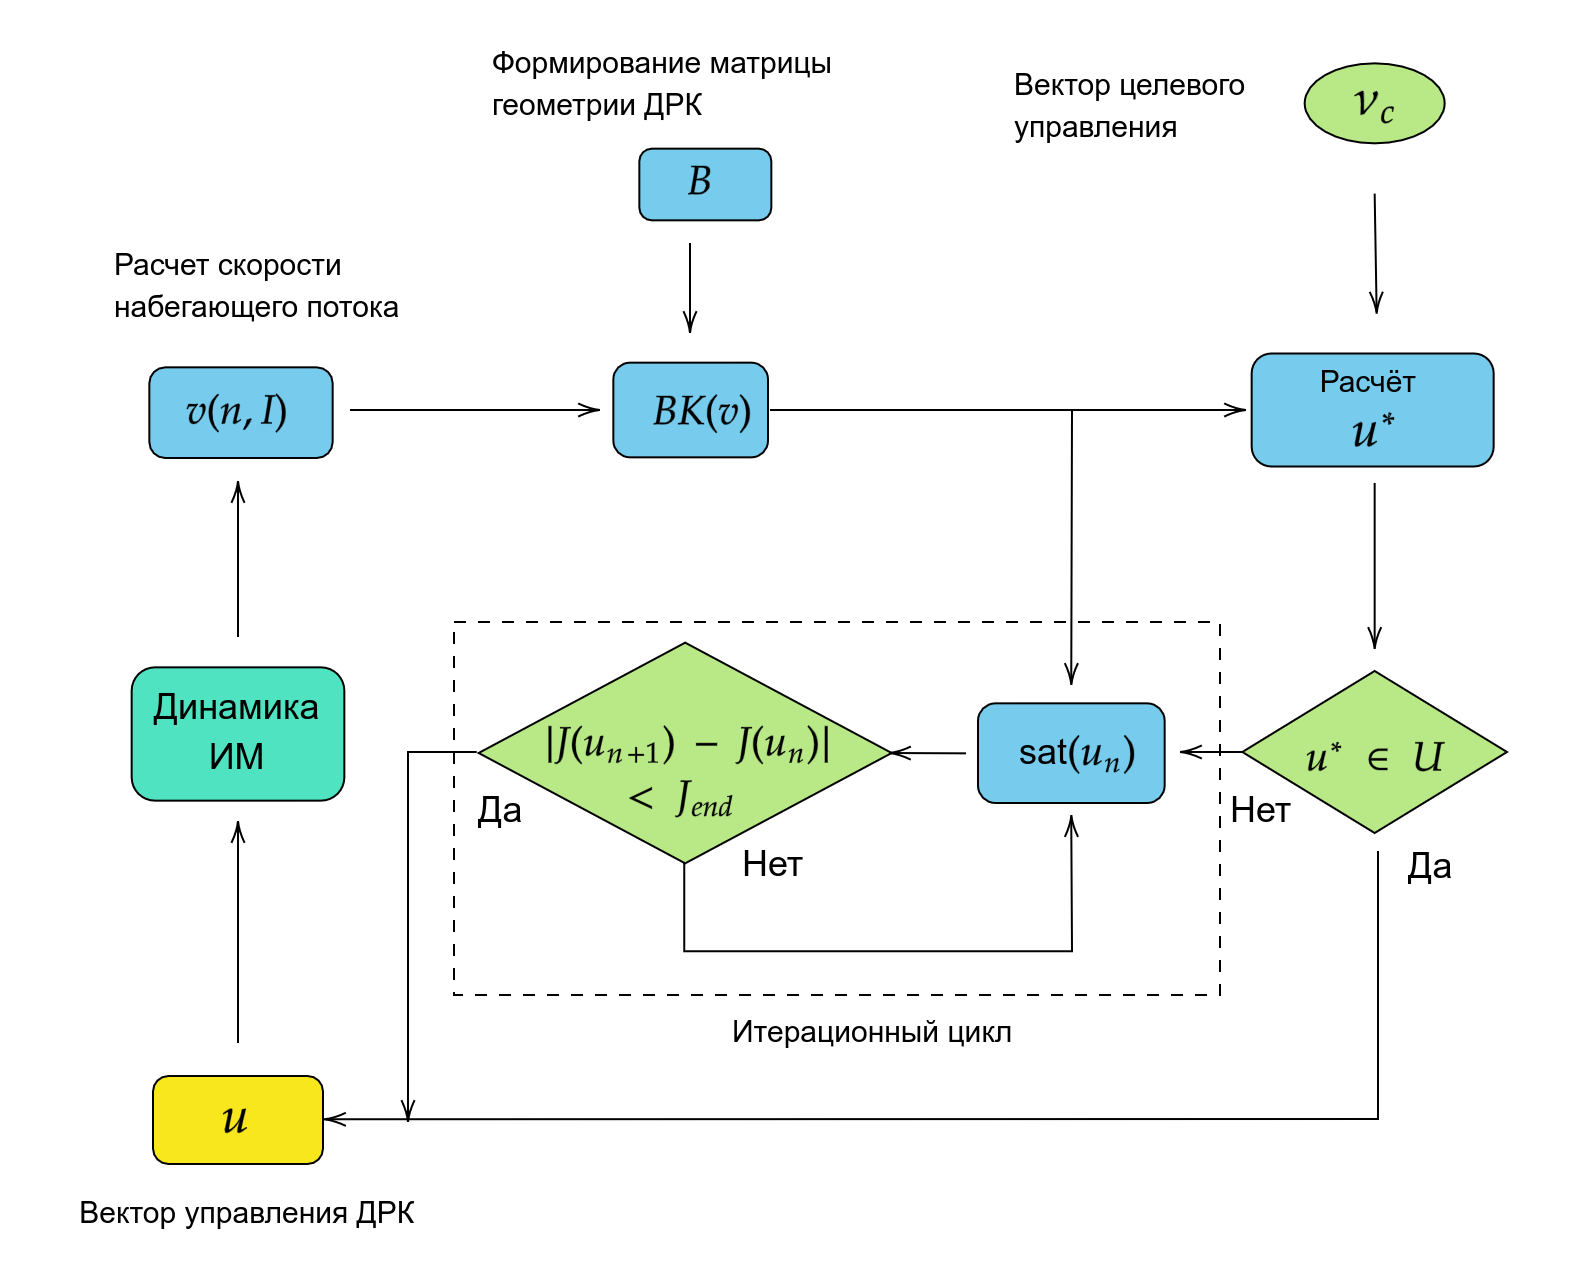
\includegraphics[width=1.0\linewidth]{allocation/Алгоритм - Блок-схема.png}
    \caption{Общая блок-схема реализации алгоритма адаптивного управления ДРК.}
    \label{fig:method_algorithm}
\end{figure}

\section{Анализ эффективности адаптивного метода управления ДРК}
В рамках исследования был проведён численный анализ эффективности представленного адаптивного метода управления ДРК на базе модели ДРК АНПА ``ММТ-300''\cite{борейко2019малогабаритный}.
Было проведено сравнительное исследование работы предлагаемого метода по сравнению с набором аналогичных методов управления в случае отсутствия набегающего потока (раздел \ref{sec:Allocation/StaticTest}).
Кроме этого было проведено сравнение поведения адаптивного метода при различных вариациях скорости (раздел \ref{sec:Allocation/SpeedTest}).
Описание модели ДРК АНПА ``ММТ-300'' (ранее ``X-300'') на которой все результаты были получены представлено в разделе \ref{ssec:Allocation/PropulsionDescription}.

\subsection{Описание модели ДРК}\label{ssec:Allocation/PropulsionDescription}
``ММТ-300'' -- автономный необитаемый подводный аппарат, который спроектирован и разработан в Институте проблем морских технологий ДВО РАН.
Он предназначен для проведения подводных работ на глубинах до 300 метров.

АНПА оснащен четырьмя симметрично расположеными относительно продольной оси ПА маршевыми движителями. 
Они установлены в корме аппарата с углом наклона относительно продольной оси ПА $\delta$.
Для возможности управления при малых скоростях (в диапазоне скоростей 0 - 1.0 м/с) он дополнительно оборудован двумя подруливающими движителями в носовой части аппарата -- одним вертикальным и одним горизонтальным.

Конструктивные параметры ДРК $L_s^x, L_s^y, L_s^z$ определяют, соответственно, проекцию расстояния от точки крепления кормовых движителей до ЦМ ПА на продольную, поперечную и нормальную оси.
В силу симметрии расположения движителей $|L_s^y| = |L_s^z|$ для всех движителей маршевой группы.
Переменные $L_{tv}$ и $L_{th}$ определяют, соответственно, расстояния от точки крепления вертикального и горизонтального подруливающего движителя до ЦМ ПА.

В качестве ССК используется BODY СК \cite{fossen2011handbook} центр которой приложен к центру водоизмещения ПА, а оси ориентированы вдоль главных осей его инерции: ось $x$ направлена вдоль продольной оси аппарата с кормы в нос, ось $y$ направлена вдоль поперечной оси аппарата от левого бока на правый, а ось $z$ достраивает СК до правосторонней.

Геометрические параметры ДРК АНПА ``ММТ-300'' указаны в таблице \ref{tab:mmt300_propulsion_param}.
Координаты каждого ИМ в ССК приведены в таблице \ref{tab:mmt300_propulsion}.
% Численные значения указанных переменных для АНПА ``ММТ-300'' указаны в таблице \ref{tab:mmt300_propulsion}.
% Положение и ориентация каждого движителя представлена в таблице \ref{tab:mmt300_propulsion}.
% В таблице \ref{tab:mmt300_propulsion} уголы $\psi$ и $\theta$ определяют отклонение вектора формирования упора движителя от продольной оси аппарата в горизонтальной и вертикальной плоскости соответственно.
% Координата в ССК определяет положение движителя в системе координат связанной с ЦМ ПА, где ось $x$ направлена вдоль продольной оси аппарата с кормы в нос, ось $y$ направлена вдоль поперечной оси аппарата от левого бока на правый и ось $z$ достраивает СК до правосторонней.

\begin{figure}[ht]
    \centering
    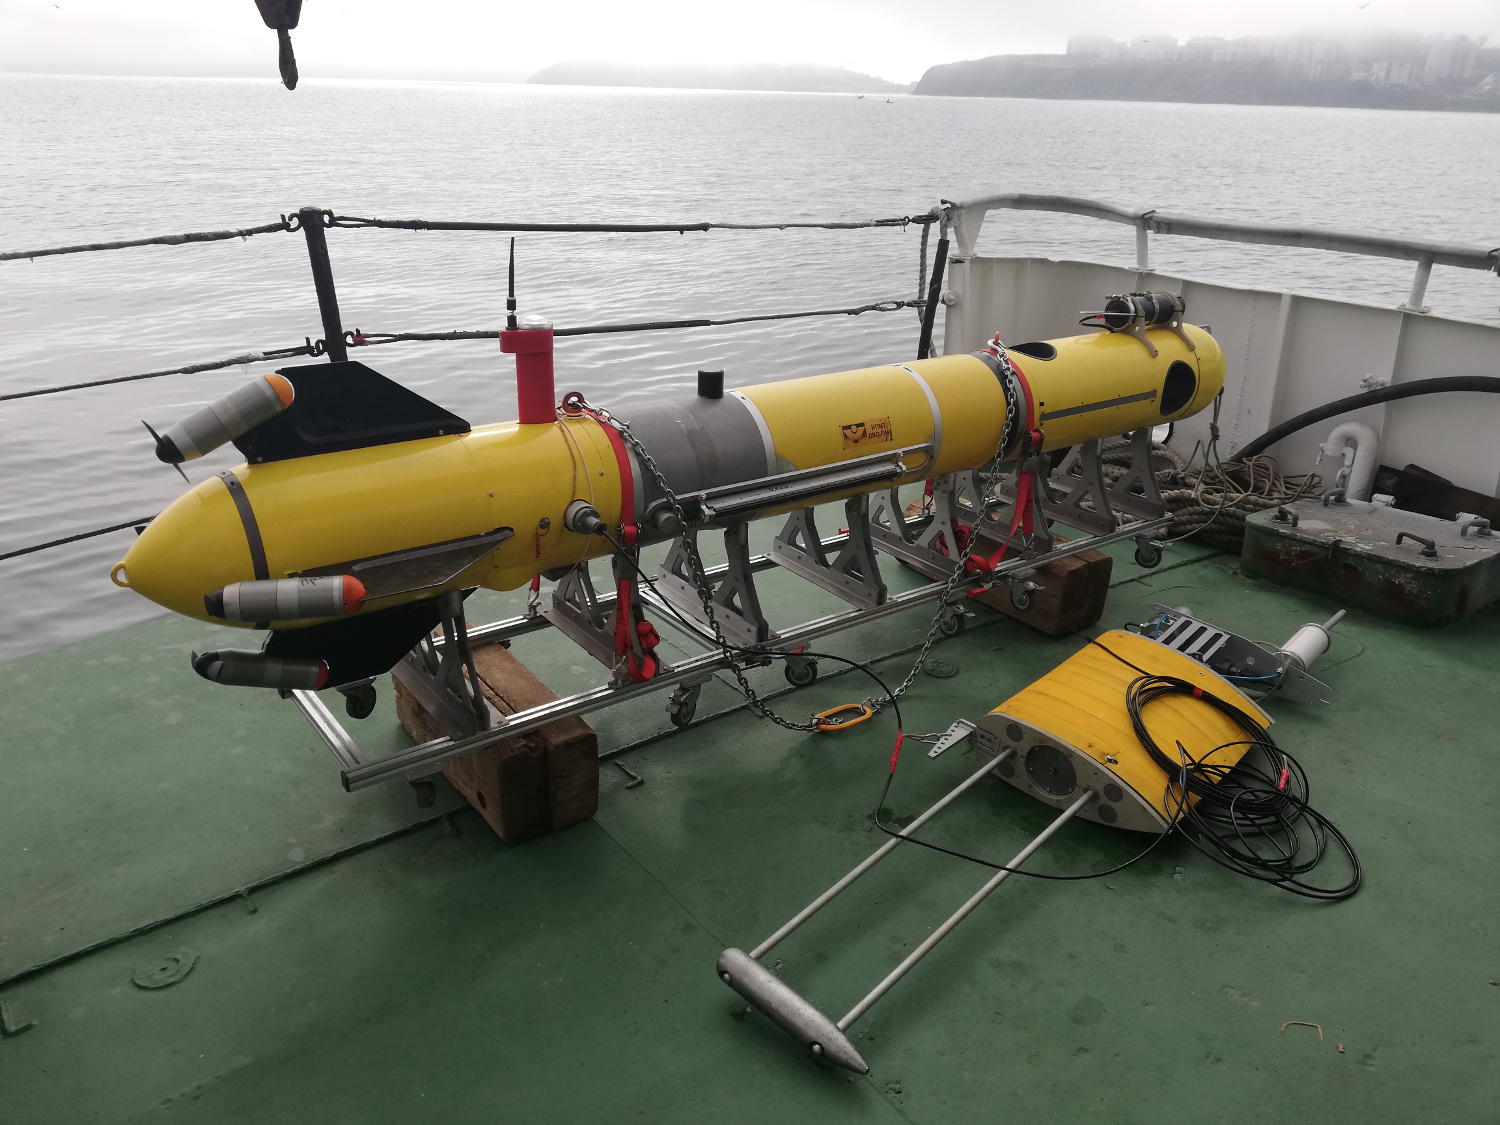
\includegraphics[width=0.8\linewidth]{allocation/Распределение - вид ММТ300.jpg}
    \caption{Общий вид аппарата АНПА ``ММТ-300''.}
    \label{fig:mmt-300}
\end{figure}

\begin{table}
    \caption{Параметры ДРК АНПА ``ММТ-300''.}
    \label{tab:mmt300_propulsion_param}
    \centering
    \begin{tabular}{ll}
        \toprule
        Наименование & Величина \\ 
        \midrule
        $\delta$ & 22.5$^{\circ}$ \\
        $L_s^x$ & 1.60 м \\
        $L_s^y$ & 0.14 м \\
        $L_{tv}$ & 0.3 м \\
        $L_{th}$ & 1.0 м \\
        \bottomrule
    \end{tabular}
\end{table}

\begin{table}
    \caption{Координаты ИМ ДРК АНПА ``ММТ-300'' в ССК.}
    \label{tab:mmt300_propulsion}
    \centering
    \begin{tabular}{lll}
        \toprule
        Наименование & \makecell[l]{Ориентация $(\psi, \theta)$, $^{\circ}$} & \makecell[l]{Положение 
        в ССК $(x,y,z)$, м} \\
        \midrule
        \multicolumn{3}{c}{Маршевые движители} \\
        \midrule
        Нижний  & (0, -$\delta$) & (-$L_s^x$,0,$L_s^y$) \\
        Верхний & (0, $\delta$)  & (-$L_s^x$,0,-$L_s^y$) \\
        Левый   & (-$\delta$, 0) & (-$L_s^x$,-$L_s^y$,0) \\
        Правый  & ($\delta$, 0)  & (-$L_s^x$,$L_s^y$,0) \\
        \midrule
        \multicolumn{3}{c}{Подруливающие движители} \\
        \midrule
        Вертикальный    & (0, 90) & ($L_{tv}$,0,0) \\
        Горизонтальный & (90, 0) & ($L_{th}$,0,0) \\
        \bottomrule
    \end{tabular}
\end{table}

Пусть управление ДРК ПА задано вектором $\vect{u} = [u_{sd},u_{su},u_{sl},u_{sr}, u_{tv},u_{th}]^T$, где переменные $u_{sd},u_{su},u_{sl},u_{sr}$ определяют упоры соответственно для нижнего, верхнего, левого и правого маршевого движителя, а переменные $u_{tv},u_{th}$ определяют упоры соответственно для вертикального и горизонтального подруливающего движителя.

Пусть управление движением ПА, в свою очередь, задано вектором $\vect{v} = [f_x,f_y,f_z,m_y,m_z]^T$, где $f_x,f_y, f_z$ -- соответствено силы вдольно продольной, поперечной и нормальной оси ССК, а $m_y,m_z$ -- моменты вокруг поперечной (``по дифференту'') и вокруг нормальной (``по крену'') оси ССК. Ось управления по $m_z$ (``по крену'') отсутствует, т.к. ПА при такой конфигурации по ней не управляем.

Матрица геометрии ДРК для конфигурации движителей представленной в таблице \ref{tab:mmt300_propulsion} в соответствии с выражением \ref{eq:propulsion_matrix} будет выглядеть следующим образом:
\begin{equation}
    \label{eq:mmt300_propulsion_matrix}
    B = 
    \begin{pmatrix}
        b_d, b_u, b_l, b_r, b_h, b_v
    \end{pmatrix}
\end{equation}
\noindent где
\begin{equation*}
    b_d = 
    \begin{pmatrix}
        \cos{\delta} \\
        0 \\
        -\sin{\delta} \\
        \cos{\delta} \cdot L_s^y - \sin{\delta} \cdot L_s^x \\
        0
    \end{pmatrix}
    ;\:
    b_u = 
    \begin{pmatrix}
        \cos{\delta} \\
        0 \\
        \sin{\delta} \\
        -\cos{\delta} \cdot L_s^y + \sin{\delta} \cdot L_s^x \\
        0
    \end{pmatrix}
\end{equation*}

\begin{equation*}
    b_l = 
    \begin{pmatrix}
        \cos{\delta} \\
        -\sin{\delta} \\
        0 \\
        0 \\
        -\cos{\delta} \cdot L_s^y - \sin{\delta} \cdot L_s^x
    \end{pmatrix}
    ;\:
    b_r = 
    \begin{pmatrix}
        \cos{\delta} \\
        \sin{\delta} \\
        0 \\
        0 \\
        \cos{\delta} \cdot L_s^y +  \sin{\delta} \cdot L_s^x
    \end{pmatrix}
\end{equation*}

\begin{equation*}
    b_h = 
    \begin{pmatrix}
        0 \\
        0 \\
        1 \\
        -L_{tv} \\
        0
    \end{pmatrix}
    ;\:
    b_v = 
    \begin{pmatrix}
        0 \\
        1 \\
        0 \\
        0 \\
        L_{th} \\
    \end{pmatrix}
\end{equation*}

Швартовная характеристика движителей АНПА ``ММТ-300'' представлена на рисунке \ref{fig:mmt-300-bollard-pull}.

\begin{figure}[ht]
    \centering
    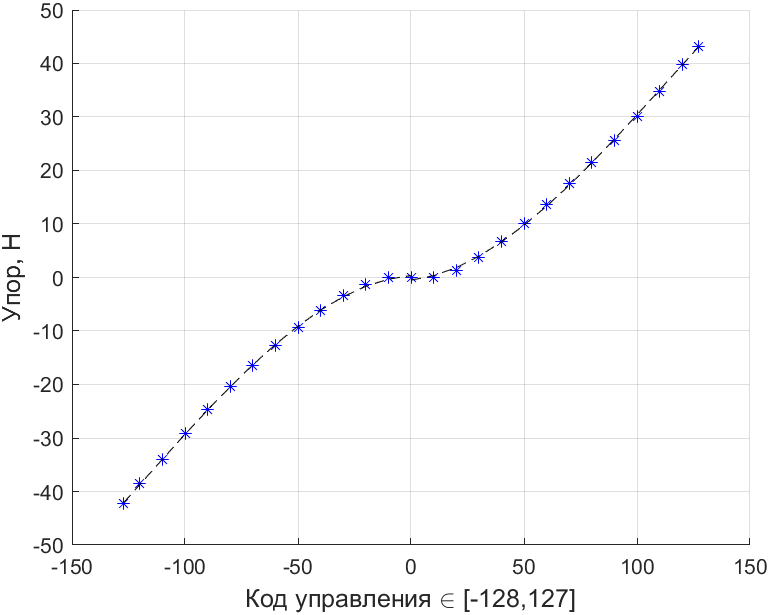
\includegraphics[width=0.8\linewidth]{allocation/MMT-300 - Швартовая характеристика.png}
    \caption{Швартовная статическая характеристика движителей АНПА ``ММТ-300''.}
    \label{fig:mmt-300-bollard-pull}
\end{figure}

\subsection{Статический сравнительный анализ работы адаптивного метода} \label{sec:Allocation/StaticTest}
Для статического сравнительного анализа работы адаптивного метода был проведен анализ результатов решения задачи управления ДРК ПА для случайного перебора вектора целевого управления движением ПА $\vect{v_r}$ \cite{kostenko2021comparative, костенко2020анализ}.

В качестве параметров сравнения различных методов управления ДРК были взяты следующие величины:
\begin{itemize}
    \item размер сформированной области допустимых значений вектора управления движением;
    \item среднее время работы метода;
    \item средняя потребляемая мощность;
    \item средня норма вектора невязки.
\end{itemize}

В качестве размера области допустимых значений вектора управления движением ПА $\vect{v_r}$ был взят объем выпуклой оболочки $\mathspace{A}$ ($n$-симплекса) построенной на семействе векторов $(\vect{\nu^b_1},\:\vect{\nu^b_2},\:,\ldots, \vect{\nu^b_k})$ которые получены следующим образом.

Пусть $(\vect{u}^l_1, \vect{u}^l_2, \ldots, \vect{u}^l_k)$ -- множество векторов управления ДРК полученых полным перебором где $u^l_i$ принимают значения $\underline{u_i}$  либо $\overline{u_i}$.
Размер множества векторов $k$ будет определен как $2^m$ где $m$ -- количество ИМ в составе ДРК.

Тогда $\vect{\nu^b_i}$ будет получен следующим выражением:
\begin{equation*}
    \vect{\nu^b_i} = B\vect{u}^*_i
\end{equation*}
\noindent где $\vect{u}^*_i$ -- вектор управления ДРК полученный путем решения задачи управления ДРК заданным методом для $\vect{v}_i$, где, в свою очередь, $\vect{v}_i$ определено следующим выражением:

\begin{equation*}
    \vect{v}_i = B \vect{u}^l_i  
\end{equation*}

Пример проекции области допустимых значений для метода линейных ограничений и фиксированной точки на оси $T_x-M_y-M_z$ представлен на рисунке \ref{fig:mmt-300-feasible-set-3d}.
Проекции областей допустимых значений на оси $Tx-My$ для всех методов представлен на рисунке \ref{fig:mmt-300-feasible-set}.

\begin{figure}[ht]
    \centering
    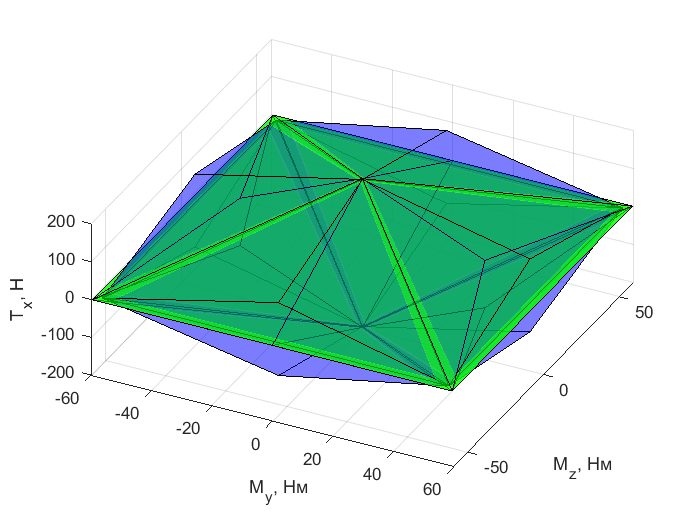
\includegraphics[width=0.8\linewidth]{allocation/ММТ-300 - область допустимых значений TxMyMz.png}
    \caption{Проекция области допустимых значений для метода линейных ограничений и фиксированной точки на оси $T_x-M_y-M_z$.}
    \label{fig:mmt-300-feasible-set-3d}
\end{figure}

\begin{figure}[ht]
    \centering
    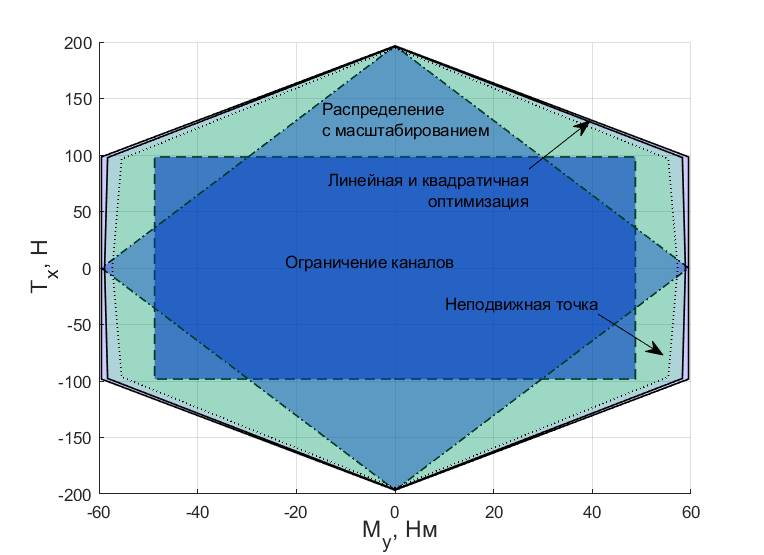
\includegraphics[width=0.8\linewidth]{allocation/ММТ-300 - область допустимых значений.png}
    \caption{Проекция области допустимых значений на оси $T_x-M_y$.}
    \label{fig:mmt-300-feasible-set}
\end{figure}


Для расчёта потребляемой мощности была использована следующая формула \cite{baldini2018constrained}:
\begin{equation*}
    P = \sum_{i=1}^p k_i t_i^{3/2}
\end{equation*}
\noindent где $k_i$ -- некоторые коэффициенты.

% \begin{notequestion}
% 	Сущность этих коэффициентов и их численное значение для сравнительного анализа не важны
% \end{notequestion}
В качестве нормы невязки управления была использована евклидова норма разности целевого и результирующего векторов управления $||\vect{s}|| =\vect{v_r} - B\vect{u^*}||$.

Все расчёты приведены в относительные единицы по каждому из параметров исследования.
В качестве базовой величины использовалось минимальное значение по каждому из параметров в отдельности.
Остальные величины были расчитаны по следующей формуле:

\begin{equation*}
    P_r = \left( \frac{P_a}{P_a^{min}} - 1 \right) * 100\%
\end{equation*}
\noindent где
\begin{itemize}
    \item $P_r$ -- значение параметра в относительных единицах;
    \item $P_a$ -- значение параметра в абсолютных единицах единицах;
    \item $P_a^{min}$ -- минимальное значение параметра при сравнении различных методов.
\end{itemize}

Результаты статического анализа представлены в таблице \ref{tab:comparison_result}.

\begin{table}[h]
    \caption{Результаты сравнительного анализа методов управления ДРК.}
    \label{tab:comparison_result}
    \centering
    \small
\begin{tabular}{lllll}
    \toprule
    Метод & Время работы,~\% & \makecell[l]{Размер  \\ области $\mathspace{A}$,~\%} & \makecell[l]{Потребляемая \\ мощность,~\%} & $||\vect{s}||$,~\% \\
    \midrule
    Фиксированное ограничение  &
    1,5 &
    \textbf{0} &
    2,3 &
    \textbf{2,6}
    \\ 
    Линейное ограничение &
    1,3 &
    22,1 &
    2,9 & 
    2,6
    \\
    Линейная оптимизация&
    \textbf{352,5}  &
    \textbf{83,2}  &
    \textbf{43,3}  &
    \textbf{0}
    \\
    Квадратичная оптимизация &
    68  &
    79,3  &
    2,1  &
    2,4
    \\
    Адаптивная оптимизация &
    \textbf{0}  &
    70,2  &
    \textbf{0}  &
    1,8 
    \\
    \bottomrule
\end{tabular}
\end{table}

\subsection{Моделирование работы адаптивного метода управления ДРК при различных скоростях набегающего потока} \label{sec:Allocation/SpeedTest}
В рамках исследования было произведено сравнение двух методов: адаптивный метод управления ДРК предлагаемый в исследовании и метод прямого управления ДРК с линейным масштабированием (раздел \ref{sssec:AllocationFix}) адаптированный для различных вариаций скорости, который реализован на АНПА ``ММТ-300''.

Для решения задачи адаптивного управления используется матрица коэффициентов влияния набегающего потока, которая, в соответствии с уравнением \ref{eq:flow_matrix}, задана следующим образом:
\begin{equation}
    \label{eq:flow_matrix_test}
    K(v) = 
    \begin{pNiceMatrix}[columns-width=auto]
       1 & 0 & 0 & 0 & 0 & 0 \\
       0 & 1 & 0 & 0 & 0 & 0 \\
       0 & 0 & 1 & 0 & 0 & 0 \\
       0 & 0 & 0 & 1 & 0 & 0 \\
       0 & 0 & 0 & 0 & e^{-c_{tv}\frac{v}{u_j}} & 0 \\
       0 & 0 & 0 & 0 & 0 &  e^{-c_{tv}\frac{v}{u_j}}\\
    \end{pNiceMatrix}
\end{equation}
\noindent где $c_{tv}, c_{th}$ -- соответственно коэффициент подавления упора вертикального и горизонтального движителя.


\subsubsection{Описание метода прямого управления ДРК с линейным масштабированием для различных типов движения}
Адаптация к смене типа движения в случае прямого управления ДРК с линейным масштабированием происходит следующим образом.
Пусть задача управления ДРК решена в соответствии с разделом \ref{sssec:AllocationFix}, т.е.:
\begin{equation*}
    \vect{u^*} = C\vect{\alpha}\vect{\nu_c}
\end{equation*}
\noindent где
\begin{itemize}
    \item $C = W^{-1}B(v)^T(B(v)W^{-1}B(v)^T)^{-1}$ -- решение оптимальной задачи управления ДРК через псевдообратную матрицу Мура-Пенроуза для случая $\mathspace{U}=\mathspace{R}$;
    \item $\vect{\alpha}$ -- вектор линейных сжимающих коэффициентов, которые обеспечивают удержание $\vect{u}^*$ внутри подмножества допустимых значений $\mathspace{U}$;
\end{itemize}

Адаптация к различным вариациям скорости движения ПА происходит за счет модификации матрицы геометрии $B(v)$ следующего вида:
\begin{equation*}
    B(v) =
    \left\{
    \begin{matrix}
        B_p, \text{ если } v < v_{\text{cruise}} \\
        B_c, \text{ если } v > v_{\text{cruise}} \\
    \end{matrix}
    \right.
\end{equation*}
\noindent $v$ -- скорость набегающего потока, $v_{\text{cruise}}$ -- параметр определяющий границу позиционного ($v < v_{\text{cruise}}$) и крейсерского ($v > v_{\text{cruise}}$) типа движения ПА, матрица $B_p$ полностью соответствует матрице \ref{eq:mmt300_propulsion_matrix}, а $B_c$, формируется путем исключения из геометрии ДРК подруливающих движителей, т.е:
\begin{equation*}
    B_c = (b_d, b_u,b_l,b_r)
\end{equation*}

\subsubsection{Методология проведения моделирования}
Было осуществено моделирование маневра по глубине, т.е. управление ДРК при продольном движении аппарата с одновременным созданием момента по каналу дифферента.
Вектор целевого управления движением ПА $\vect{\nu_c}$ в BODY ССК выглядит следующим образом: $\vect{\nu_c} \equiv \vect{f}^b_c = [f_x, f_y, f_z, m_y, m_z]$, где $f_x,\: f_y,\: f_z$ -- соответственно, проекция целевой силы на продольную, поперечную и нормальную ось, а $m_y,\: m_z$ -- сответствующие проекции целевого момента.
В моделируемом случае целевая сила определяется следующим выражением:

\begin{equation*}
    \vect{f}^b_c = 
    \begin{pmatrix}
        c_xv^2 \\
        0 \\
        0 \\
        m_y^0 \\
        0
    \end{pmatrix}
\end{equation*}
\noindent где $c_x$ -- коэффицент лобового сопротивления движению ПА, $v$ -- продольная скорость движения ПА, $m_y^0$ -- фиксированный момент по дифференту сформированный СУ ПА.

Для моделирования были приняты следующие коэффициенты:
\begin{itemize}
    \item $c_x$ -- 35,0 Н $\cdot$ м/с;
    \item $m_y^0$ -- 40,0 Нм;
\end{itemize}

Весовые коэффициенты итерационной формулы поиска адаптивного управления ДРК \ref{eq:Allocation/FixedMethod} представлены в таблице \ref{tab:weight_coeff}.
Численные параметры расчёта матрицы коэффициентов влияния набегающего потока \ref{eq:flow_matrix_test} представлены в таблице \ref{tab:matrix_flow_coeff}.

\begin{table}
    \caption{Весовые коэффициенты для адаптивного управления ДРК.}
    \label{tab:weight_coeff}
    \centering
    \begin{tabular}{ll}
        \toprule
        Наименование & Величина \\
        \midrule
        $\epsilon$ & 0.8 \\
        $Q_{\nu}$ & $\text{diag}([0,6;\:0,0;\:0,0;\:2,25;\:0,0])$ \\
        $Q_{n}$  & $\text{diag}([0,4;\:0,4;\:0,4;\:0,4;\:0,4])$ \\
        \bottomrule
    \end{tabular}
\end{table}

\begin{table}
    \caption{Параметры расчёта матрицы $K(v)$.}
    \label{tab:matrix_flow_coeff}
    \centering
    \begin{tabular}{lll}
        \toprule
        Описание & Обозначение & Величина \\
        \midrule
        Коэффициент подавления упора & $c$ & 2.0 \\
        Диаметр винта & $D$ & 0.14 м \\
        Плотность воды & $\rho$ & 1000 кг/м$^3$ \\
        \bottomrule
    \end{tabular}
\end{table}

Результаты распределения упоров методом прямого управления ДРК с масштабированием в диапазоне скоростей от 0 до 2.5 м/с представлены на рисунке \ref{fig:mmt-300-allocation-fix-thrust}.
В свою очередь на рисунке \ref{fig:mmt-300-allocation-fix-force} показаны целевые и фактические силы которые были при этом.
Аналогичные данные для адаптивного метода управления ДРК представлены на рисунках \ref{fig:mmt-300-allocation-optimal-thrust} и \ref{fig:mmt-300-allocation-optimal-force} соответственно.

\begin{figure}[ht]
    \centering
    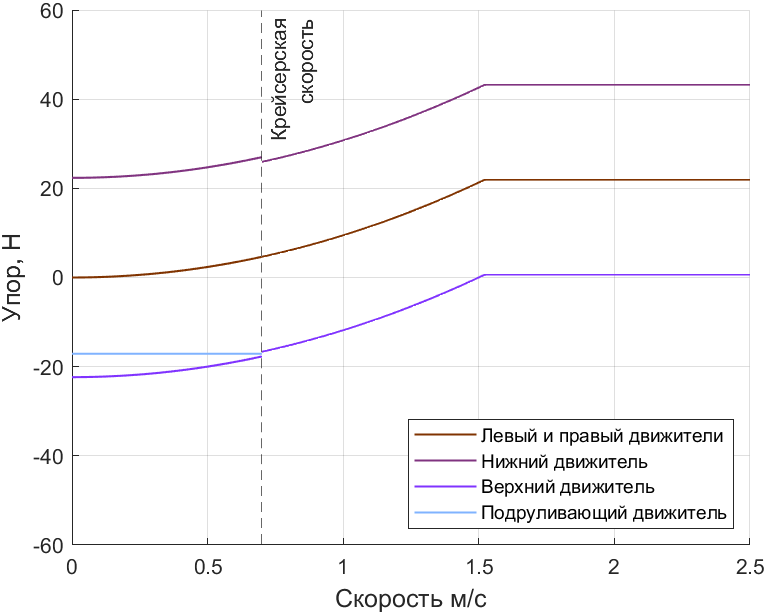
\includegraphics[width=0.8\linewidth]{allocation/Результат ММТ300 - Стандартный упоры.png}
    \caption{Распределение упоров методом прямого управления ДРК с масштабированием.}
    \label{fig:mmt-300-allocation-fix-thrust}
\end{figure}

\begin{figure}[ht]
    \centering
    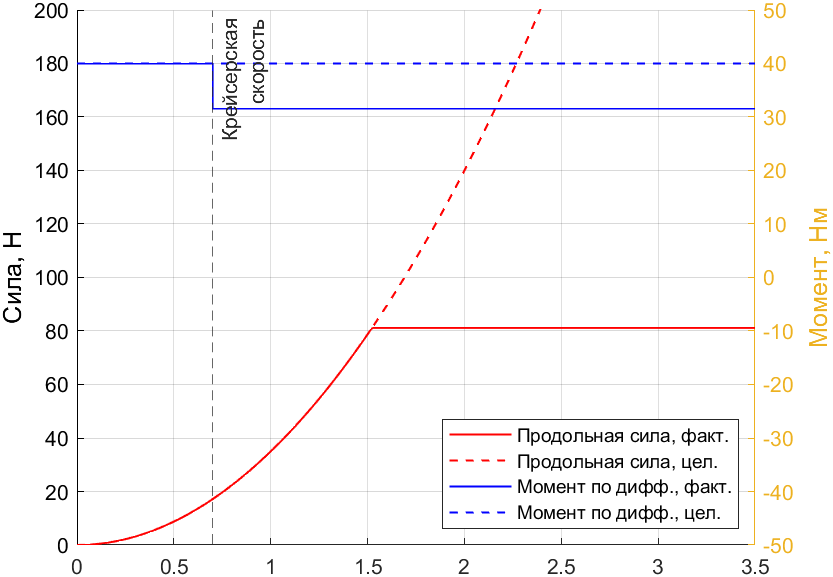
\includegraphics[width=0.8\linewidth]{allocation/Результат ММТ300 - Стандартный силы.png}
    \caption{Силы и моменты при прямом управлении с масштабированием.}
    \label{fig:mmt-300-allocation-fix-force}
\end{figure}

\begin{figure}[ht]
    \centering
    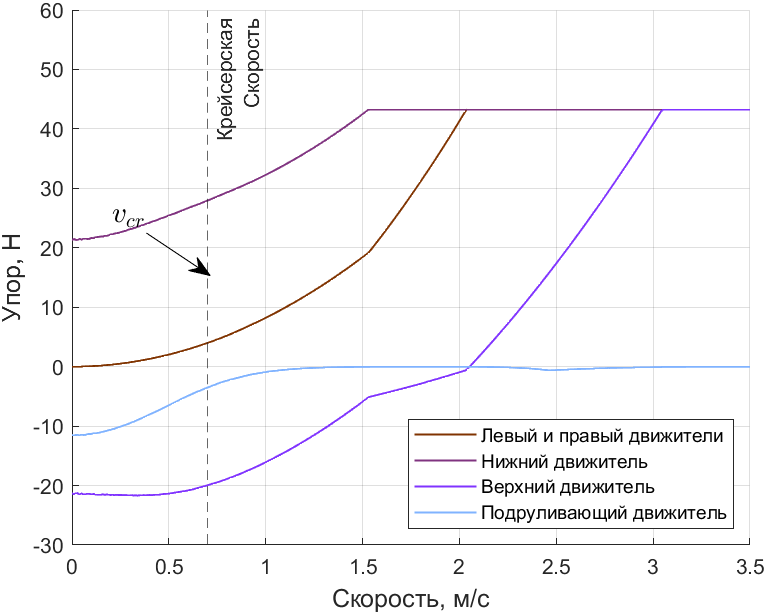
\includegraphics[width=0.8\linewidth]{allocation/Результат ММТ300 - Адаптивный Упоры.png}
    \caption{Распределение упоров адаптивным методом.}
    \label{fig:mmt-300-allocation-optimal-thrust}
\end{figure}

\begin{figure}[ht]
    \centering
    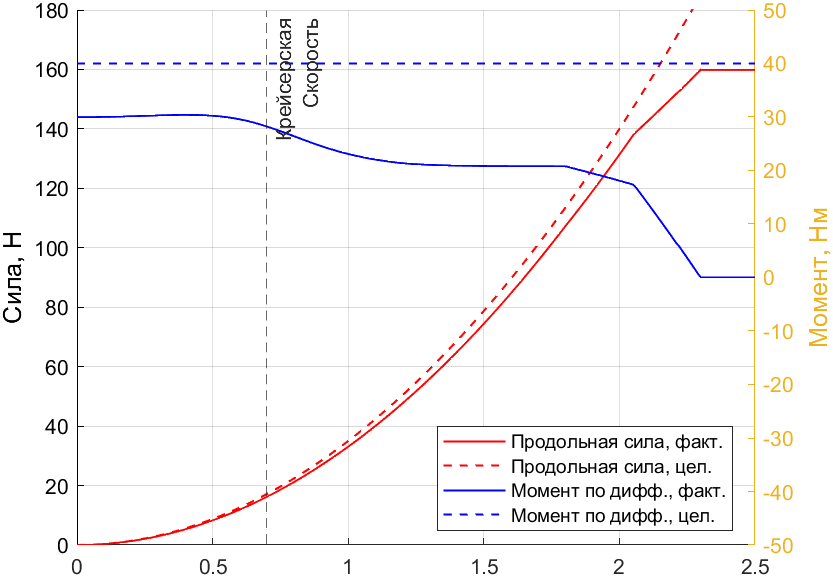
\includegraphics[width=0.8\linewidth]{allocation/Результат ММТ300 - Адаптивный силы.png}
    \caption{Силы и моменты при адаптивном методе.}
    \label{fig:mmt-300-allocation-optimal-force}
\end{figure}

\section{Прикладная реализация разработанного метода} \label{sec:Allocation/Software}
Структура современных СУ АНПА разрабатываемых в ИПМТ ДВО РАН имеет модульный принцип построения \cite{борейко2019система, инзарцев2015реконфигурируемая}, т.е. представляет собой совокупность независимых функционально завершенных исполняемых файлов взаимодействие между которыми происходит заранее сформированными сообщениями.
Взаимодействие между модулями обеспечивается системой передачи сообщений IPC, подробности работы которой описаны в статье \cite{pavin2016reconfigurable}.

На рисунке \ref{fig:software_old} показано структурное описание текущей реализции СУ АНПА ДВО РАН в части управления движением.
На рисунке изображены следующие модули СУ:
\begin{itemize}
    \item ``Navigation'' -- модуль, комплексирующий навигационные данные от всех датчиков АНПА и публикующий самые лучшие данные в стандартном формате, где $\vect{p}^n_{b/n}$ -- положение АНПА в некоторой заданной инерциальной СК, $\vect{v}^n_{b/n}$ -- скорость АНПА в этой СК, а $\vect{v}^b_{b}$ -- скорость движения АНПА в ССК.
    \item ``Mission'' -- модуль который обеспечивает стратегический уровень управления движием АНПА, т.е. он формирует список целевых координат в географической СК вдоль которых последовательно должен пройти АНПА и перечень устройств которые в данный момент времени должны быть активированы.
    \item ``Tack'' -- совокупность модулей обеспечивающих тактическое управление, т.е. формирующие траекторное управление движением АНПА между заданными географическими точками общего маршрута движения.
    \item ``Motion'' -- модуль оперативного управления движением АНПА, который обеспечивает управление движением независимо по всем доступным осям в некототорой локальной СК на основе целевых параметров поставляемых модулем ``Tack'' и текущего положения АНПА. Так же этот модуль обеспечивает управление ДРК на основе швартовных характеристик исполняемых механизмов.
\end{itemize}

\begin{figure}[ht]
    \centering
    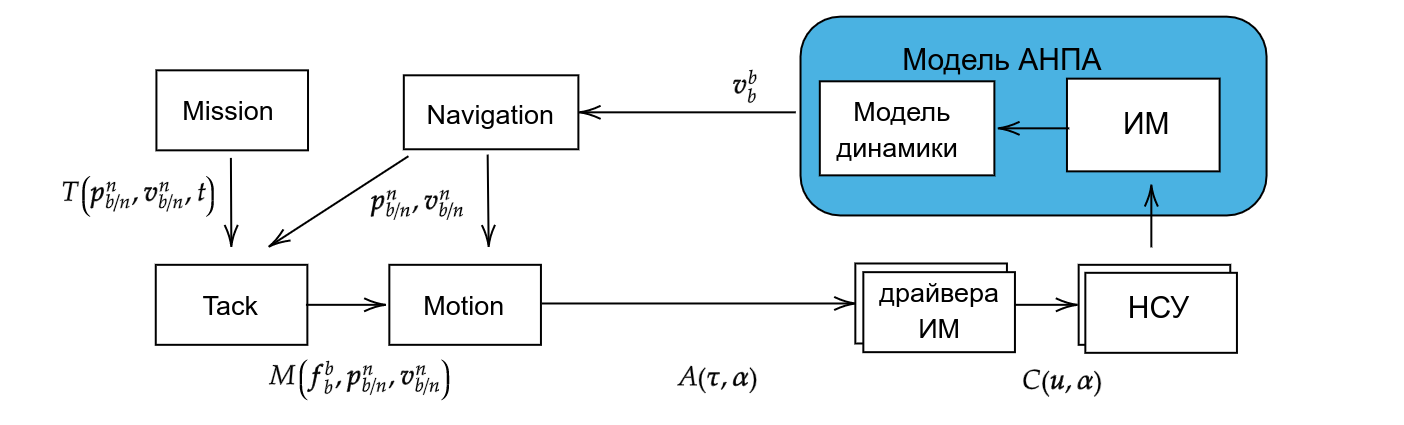
\includegraphics[width=1.0\linewidth]{allocation/Алгоритм - Реализация старая.png}
    \caption{Структурное представление текущей реализации СУ АНПА ИПМТ ДВО РАН.}
    \label{fig:software_old}
\end{figure}

В рамках исследования была предложена новая структура СУ АНПА изображённая на рисунке \ref{fig:software_new}.
Её особенность заключается в том что добавляется новый модуль ``Propulsion'' задачей которого является адаптивное распределение управляющего воздействия на базе знания модели исполнительных механизмов.
Программный модуль потребляет обобщенный вектор сил и моментов $\vect{f_b^b}$, который был сформирован модулем ``Motion''.
Модуль поставляет вектор команд управления отдельными исполнтельными элементами на вход соответствующих драйверов.
Так же исходящим параметром модуля является скорость набегающего потока, т.е. скорость АНПА в ССК.
При этом от модуля навигации он потребляет тот же вектор скорости, но в скомплексированном виде.
Общая структурная схема модуля ``Propulsion'' представлена на рисунке \ref{fig:propulsion-diagram}.

\begin{figure}[ht]
    \centering
    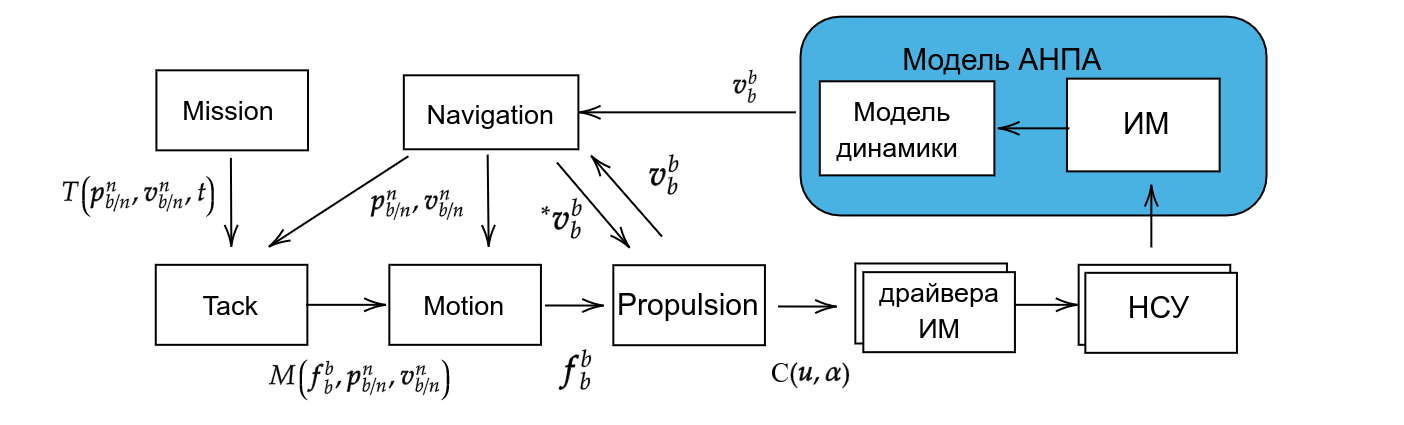
\includegraphics[width=1.0\linewidth]{allocation/Алгоритм - Реализация новая.png}
    \caption{Структурное представление предлагаемой реализации СУ АНПА ИПМТ ДВО РАН.}
    \label{fig:software_new}
\end{figure}

\begin{figure}[ht]
    \centering
    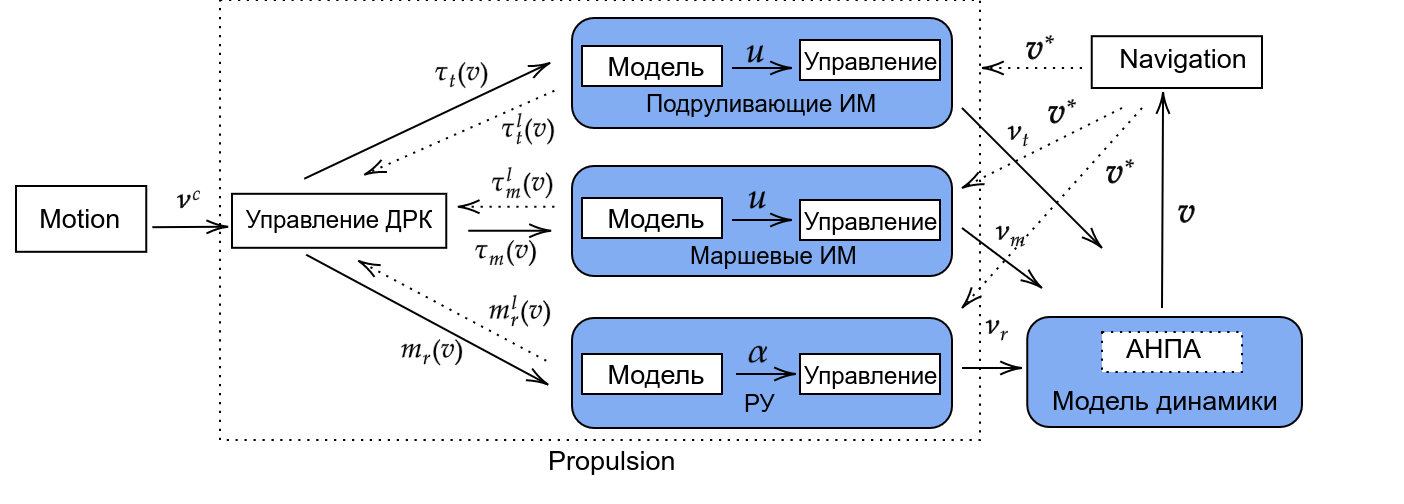
\includegraphics[width=1.0\linewidth]{allocation/Алгоритм - Реализация propulsion.png}
    \caption{Общая структурная схема модуля ``Propulsion''.}
    \label{fig:propulsion-diagram}
\end{figure}


\section{Выводы по главе 4}
Предложен новый алгоритм управления ДРК подводного аппарата, который учитывает особенности работы ИМ ДРК в набегающем потоке и способен адаптивно перераспределять управляющие воздействия при вариациях скорости.
При этом поставщиком данных о скорости набегающего потока может быть сам ДРК ПА путем анализа параметров работы маршевых движителей по закономерностям которые были получены в главе \ref{ch:Velocity}.

Показано что предложеное решение метода управления ДРК обеспечивает более высокую скорость работы по сравнению со стандартными подходами к решению задачи управления ДРК через формирование линейной и квадратичной оптимальной задачи при сопосповимой области допустимых значений.

Показано что предлагаемый алгоритм адаптивного управления ДРК позволяет плавно выключать подруливающий движитель из управления движением ПА.
По сравнению с используемым в АНПА ``ММТ-300'', предлагаемый метод позволяет обеспечивать более широкий диапазон управления и позволяет удерживать заданный момент при более высоких значениях целевой скорости.

Показан механизм модификации модульной СУ АНПА ``ММТ-300'' для прикладной реализации алгоритма адаптивного управления ДРК с идентификацией набегающего потока по параметрам работы маршевых движителей.